% !TEX program = xelatex
% 任务二独立论文：AlexNet + Fashion-MNIST
\documentclass[12pt,a4paper,fontset=fandol]{ctexart}
\usepackage[a4paper,margin=2.4cm]{geometry}
\usepackage{graphicx}
\usepackage{booktabs}
\usepackage{float}
\usepackage{caption}
\usepackage{array}
\usepackage{amsmath}
\usepackage{amssymb}
\usepackage{enumitem}
\usepackage{setspace}
\usepackage{hyperref}
\hypersetup{hidelinks}

\captionsetup{font=small, labelsep=quad}
\graphicspath{{./}{../../report/}{../../task2_alexnet_fmnist/outputs/}}
\renewcommand{\arraystretch}{1.3}
\setlength{\parindent}{2em}
\setlength{\emergencystretch}{3em}
\numberwithin{figure}{section}
\numberwithin{table}{section}
\numberwithin{equation}{section}
\onehalfspacing
\pagestyle{plain}

\ctexset{
  section/format = \zihao{4}\heiti\raggedright,
  section/beforeskip = {1ex plus 0.2ex},
  section/afterskip = {0.8ex plus 0.2ex},
  subsection/format = \zihao{-4}\heiti\raggedright,
  subsubsection/format = \zihao{-4}\kaishu\raggedright
}

\begin{document}

% ===================== 封面 =====================
\begin{titlepage}
\centering
\vspace*{1.5cm}
{\Large 本科毕业论文（设计）}\\[1.5cm]
{\Huge\bfseries 人工智能综合实训 II}\\[0.6cm]
{\LARGE\bfseries 任务二实训论文}\\[1.5cm]
{\Large\bfseries 基于 AlexNet 的 Fashion-MNIST 服饰图像分类研究}\\[2cm]
{\large
\renewcommand{\arraystretch}{1.7}
\begin{tabular}{rl}
\textbf{学\qquad 院：} & 人工智能与低空技术学院 \\
\textbf{专\qquad 业：} & 人工智能 \\
\textbf{小组成员：} & 雷正（202434610309）、蔡铭飞（202434610301）、 \\
                    & 冼嘉谦（202434610326） \\
\textbf{指导教师：} & 赵静 \\
\textbf{提交日期：} & 2026 年 6 月 \\
\end{tabular}}
\vfill
\end{titlepage}

% ===================== 原创性声明 =====================
\thispagestyle{empty}
\begin{center}{\large\bfseries 华南农业大学本科毕业论文（设计）原创性声明}\end{center}
\vspace{0.5em}
\par 本人郑重声明：所呈交的毕业论文（设计），是本人在导师的指导下，独立进行研究工作所取得的成果。
除文中已经注明引用的内容外，本论文不包含任何其他个人或集体已经发表或撰写过的作品成果。对本文的研究
做出重要贡献的个人和集体，均已在文中以明确方式标明。本人完全意识到本声明的法律结果由本人承担。
\vspace{1.2cm}
\par\hfill 作者签名：\rule{3cm}{0.4pt}\qquad 日期：\quad\ 年\ \quad 月\ \quad 日\hspace{1cm}
\vspace{2cm}

\begin{center}{\large\bfseries 华南农业大学本科毕业论文（设计）使用授权声明}\end{center}
\vspace{0.5em}
\par 本人完全了解学校有关保留、使用毕业论文（设计）的规定，同意学校保留并向国家有关部门或机构送交
毕业论文（设计）的复印件和电子版，允许毕业论文（设计）被查阅和借阅。学校可以将本毕业论文（设计）的
全部或部分内容编入有关数据库进行检索，可以采用影印、缩印或扫描等复制手段保存和汇编毕业论文（设计）。
\vspace{1.2cm}
\par\hfill 作者签名：\rule{3cm}{0.4pt}\qquad 指导教师签名：\rule{3cm}{0.4pt}\hspace{1cm}
\par\hfill 日期：\quad\ 年\ \quad 月\ \quad 日\qquad\quad 日期：\quad\ 年\ \quad 月\ \quad 日\hspace{1cm}
\newpage

% ===================== 摘要 =====================
\begin{center}{\Large\bfseries 摘\quad 要}\end{center}
\par 图像分类是深度学习中的典型任务。本文以 Fashion-MNIST 服饰图像数据集为研究对象，基于 PyTorch 基础
模块逐层构建 AlexNet 卷积神经网络，不调用任何预置 AlexNet 模型，完成数据加载、预处理、训练、验证、
测试和误差分析流程。针对 Fashion-MNIST 图像尺寸较小、类别间相似度较高等特点，本文将 $28\times28$ 灰度
图像放大至 $224\times224$，并在主模型中采用 BatchNorm、余弦退火学习率调度和数据增强等训练策略。

\par 实验结果表明，主模型在测试集上取得 94.38\% 的准确率和 0.9437 的宏平均 F1。混淆矩阵和分类样例显示，
模型对裤子、包、鞋类等区分度较高的类别识别效果较好，而 T 恤、套衫、外套和衬衫等上装类别之间仍存在
较明显混淆。进一步的消融实验表明，充分训练和 BatchNorm 对模型性能提升具有较大作用；复杂度对比显示，
AlexNet 在低分辨率灰度图像任务上存在一定参数和计算冗余。本文还通过 Focal Loss 对照和 Grad-CAM 可视化
分析模型关注区域，进一步讨论上装类别误差的来源。

\par\vspace{1ex}
\noindent\textbf{关键词：}深度学习；卷积神经网络；AlexNet；Fashion-MNIST；图像分类；Grad-CAM

\newpage
\begin{center}{\Large\bfseries Abstract}\end{center}
\par Image classification is a representative task in deep learning. This paper studies the Fashion-MNIST dataset
and builds an AlexNet convolutional neural network layer by layer using basic PyTorch modules, without calling any
predefined AlexNet model. The complete workflow includes data loading, preprocessing, training, validation, testing
and error analysis. Considering the small image size and high inter-class similarity of Fashion-MNIST, the original
$28\times28$ grayscale images are resized to $224\times224$. BatchNorm, cosine annealing and data augmentation are
used in the main model.

\par The experimental results show that the main model achieves a test accuracy of 94.38\% and a macro-F1 score of
0.9437. The confusion matrix and prediction samples indicate that the model performs well on visually distinctive
classes such as trousers, bags and shoes, while confusion remains among upper-body clothing categories such as
T-shirts, pullovers, coats and shirts. Further ablation experiments show that sufficient training and BatchNorm
make important contributions to model performance. Complexity comparison also indicates that AlexNet has certain
parameter and computation redundancy on low-resolution grayscale images. In addition, Focal Loss comparison and
Grad-CAM visualization are used to further analyze the source of errors in upper-body clothing categories.

\par\vspace{1ex}
\noindent\textbf{Keywords:} deep learning; convolutional neural network; AlexNet; Fashion-MNIST; image classification; Grad-CAM

\newpage
\tableofcontents
\newpage

% ===================== 第一章 引言 =====================
\section{引言}

\subsection{研究背景与意义}
图像分类是计算机视觉中的基础任务，也是深度学习方法最早取得显著突破的方向之一。卷积神经网络通过局部
连接、权值共享和层次化特征提取机制，能够从图像中逐级学习边缘、纹理、局部形状和高层语义信息，相比完全
连接网络更适合处理具有空间结构的视觉数据。随着计算能力、数据规模和训练技巧的发展，卷积神经网络已经
成为图像识别、目标检测、医学影像分析和工业视觉检测等任务中的重要模型。

AlexNet 在 ImageNet 图像分类任务中的成功推动了深度卷积网络的快速发展。其结构包含多层卷积、池化、ReLU
激活、局部响应归一化、Dropout 和全连接分类器，集中体现了早期深度视觉模型的关键设计。虽然当前更深或更
轻量的网络结构已经广泛应用，但 AlexNet 仍然适合作为理解卷积网络基本机制的经典模型。逐层实现 AlexNet，
而不是直接调用预置模型，可以更清楚地理解输入尺寸变化、卷积核设置、特征图尺寸、参数量和训练策略之间的
关系。

Fashion-MNIST 是 MNIST 的替代性基准数据集，由 10 类服饰图像构成。相比手写数字图像，服饰图像类别之间
存在更高的视觉相似性，特别是 T 恤、套衫、外套和衬衫等上装类别在低分辨率灰度图中边界较模糊。该数据集
规模适中、类别均衡、训练成本可控，既适合验证卷积神经网络的基本分类能力，也适合分析模型在细粒度视觉
差异不足时的错误类型。

本研究在 Fashion-MNIST 上逐层构建 AlexNet，并围绕训练策略、组件消融、模型复杂度和可解释性展开实验，
具有两方面意义。其一，实验能够展示深度图像分类从数据预处理、模型实现、训练验证到测试评估的完整流程；
其二，通过 BatchNorm、数据增强、Focal Loss、复杂度对比和 Grad-CAM 可视化，可以进一步分析模型性能来源
和误差成因，避免只以单一准确率评价模型效果。

\subsection{国内外研究现状}
卷积神经网络的发展经历了从浅层结构到深层结构、从单纯提升精度到兼顾效率与可解释性的过程。LeCun 等
(1998)提出的 LeNet 展示了卷积、池化和共享权重在手写字符识别中的有效性，为后续视觉网络奠定了基础。
Krizhevsky 等(2012)提出的 AlexNet 在大规模 ImageNet 分类任务上显著提升了识别性能，证明了深层卷积网络
在大规模视觉数据上的表达能力。随后，VGG 通过堆叠小卷积核研究网络深度对性能的影响，ResNet 则利用残差
连接缓解深层网络训练退化问题，使更深网络的训练成为可能。

在训练策略方面，早期 AlexNet 使用 ReLU 激活提升非线性表达和训练效率，并结合 Dropout 缓解全连接层过拟合。
Srivastava 等(2014)系统研究了 Dropout 对过拟合的抑制作用。Ioffe 和 Szegedy(2015)提出 Batch Normalization，
通过标准化中间层输入分布稳定训练过程，常用于替代或弱化早期网络中的局部响应归一化。数据增强也是图像
分类中常用的正则化手段，可通过随机翻转、旋转、裁剪等方式提高模型对输入扰动的鲁棒性。

在数据集方面，MNIST 长期作为图像分类入门基准，但其类别结构较简单，许多模型容易取得较高准确率。Xiao 等
(2017)提出 Fashion-MNIST，希望提供一个与 MNIST 接口相近但更具挑战性的服饰图像基准。Fashion-MNIST 中
上装类别形态相近，低分辨率灰度图缺乏颜色和纹理细节，因此比手写数字更适合检验模型对细粒度形状差异的
表达能力。围绕该数据集，研究者通常比较传统 CNN、VGG/ResNet 类模型和轻量网络在准确率、参数量和推理效率
之间的取舍。

在误差分析和模型解释方面，仅报告测试准确率难以说明卷积网络真正依赖哪些图像区域进行判断。Lin 等(2017)
提出的 Focal Loss 通过降低易分样本权重，使模型更关注难分类样本，常用于类别不平衡或难样本较多的视觉任务。
Selvaraju 等(2017)提出 Grad-CAM，通过梯度加权的类激活映射展示模型关注区域，为分析卷积神经网络预测依据
提供了可视化工具。本文在主模型训练之外引入 Focal Loss 对照和 Grad-CAM 可视化，目的在于结合混淆矩阵讨论
上装类别误差来源，而不是只比较总体准确率。

\subsection{研究内容与分工}
本文围绕 Fashion-MNIST 十分类任务开展研究，主要工作包括：逐层实现 AlexNet 网络结构，构建数据加载与
训练流程，在测试集上评估模型性能，利用混淆矩阵和预测样例分析错误类型，并通过组件消融、复杂度对比、
Focal Loss 对照和 Grad-CAM 可视化讨论模型性能来源。小组成员分工如表~\ref{tab:team} 所示。

\begin{table}[H]
  \centering
  \caption{小组成员分工表}
  \label{tab:team}
  \begin{tabular}{>{\centering\arraybackslash}m{3cm} >{\centering\arraybackslash}m{2cm} m{8cm}}
    \toprule
    学号 & 姓名 & 主要分工 \\
    \midrule
    202434610309 & 雷正 & 实验结果复核、报告内容整理与复现说明 \\
    202434610301 & 蔡铭飞 & AlexNet 网络实现、模型训练、评估与可视化分析 \\
    202434610326 & 冼嘉谦 & 图表整理、PPT 制作、论文排版与汇报 \\
    \bottomrule
  \end{tabular}
\end{table}

% ===================== 第二章 理论基础 =====================
\section{理论基础}

\subsection{卷积神经网络}
卷积神经网络通过卷积核在局部感受野上滑动提取特征。设输入特征图为 $X$，卷积核为 $W$，输出特征图可表示为
\begin{equation}
Y_{i,j,k}=\sum_{c}\sum_{u}\sum_{v}W_{u,v,c,k}X_{i+u,j+v,c}+b_k.
\end{equation}
池化层通过局部下采样降低空间分辨率并增强平移鲁棒性，ReLU 激活函数则提供非线性表达能力。

与全连接网络相比，卷积神经网络的核心优势在于局部连接和权值共享。局部连接使模型只在有限感受野内提取局部
模式，符合图像中边缘、纹理和局部形状逐级组合的特点；权值共享则使同一卷积核能够在整幅图像上检测相同模式，
显著减少参数量并增强平移等变性。随着网络层数加深，浅层卷积通常捕捉边缘和简单纹理，中间层逐步组合局部形状，
高层特征则更接近类别判别所需的语义结构。

池化层在卷积网络中承担降采样和局部不变性建模作用。最大池化保留局部区域中响应最强的特征，有助于减小输入
微小平移带来的影响，同时降低后续层的计算量。ReLU 激活函数可表示为
\begin{equation}
\mathrm{ReLU}(x)=\max(0,x),
\end{equation}
它能够引入非线性并缓解 Sigmoid、Tanh 等激活在深层网络中常见的梯度饱和问题。对于 Fashion-MNIST 这类低分辨率
灰度图像，卷积网络需要在有限像素细节中提取服饰轮廓、开口形状和局部边界差异，因此卷积核尺度、池化次数和
分类器容量都会影响最终识别效果。

\subsection{AlexNet 结构}
AlexNet 由五个卷积层和三个全连接层组成。原始 AlexNet 使用局部响应归一化（LRN）和 Dropout 等组件。本文
基于 Fashion-MNIST 的单通道灰度输入，将首层输入通道改为 1，输出类别数改为 10，并保留五个卷积块和三层
全连接分类器的基本结构。主模型中采用 BatchNorm 替代 LRN，以提升训练稳定性。

原始 AlexNet 面向 ImageNet 彩色图像设计，输入为三通道大尺寸图像，最终分类类别数为 1000。本文任务为
Fashion-MNIST 十分类，输入为单通道灰度图像，因此网络实现需要做两处基本适配：第一，将第一层卷积的输入通道
由 3 改为 1；第二，将最后一层全连接输出维度改为 10。除此之外，本文保留 AlexNet 五个卷积层和三层全连接层的
主体结构，使实验能够集中考察经典 AlexNet 结构在低分辨率服饰图像上的表现。

由于 AlexNet 的全连接分类器规模较大，当输入被调整为 $224\times224$ 后，最后一个卷积块输出约为
$256\times6\times6$，展平后进入 4096 维全连接层。大量参数集中在分类器部分，这一设计有利于提高模型容量，
但也可能在 Fashion-MNIST 这种规模适中、图像信息较简单的数据集上造成计算冗余。因此，本文不仅报告主模型
精度，还专门进行复杂度对比，以讨论模型能力和计算代价之间的关系。

\begin{figure}[H]
  \centering
  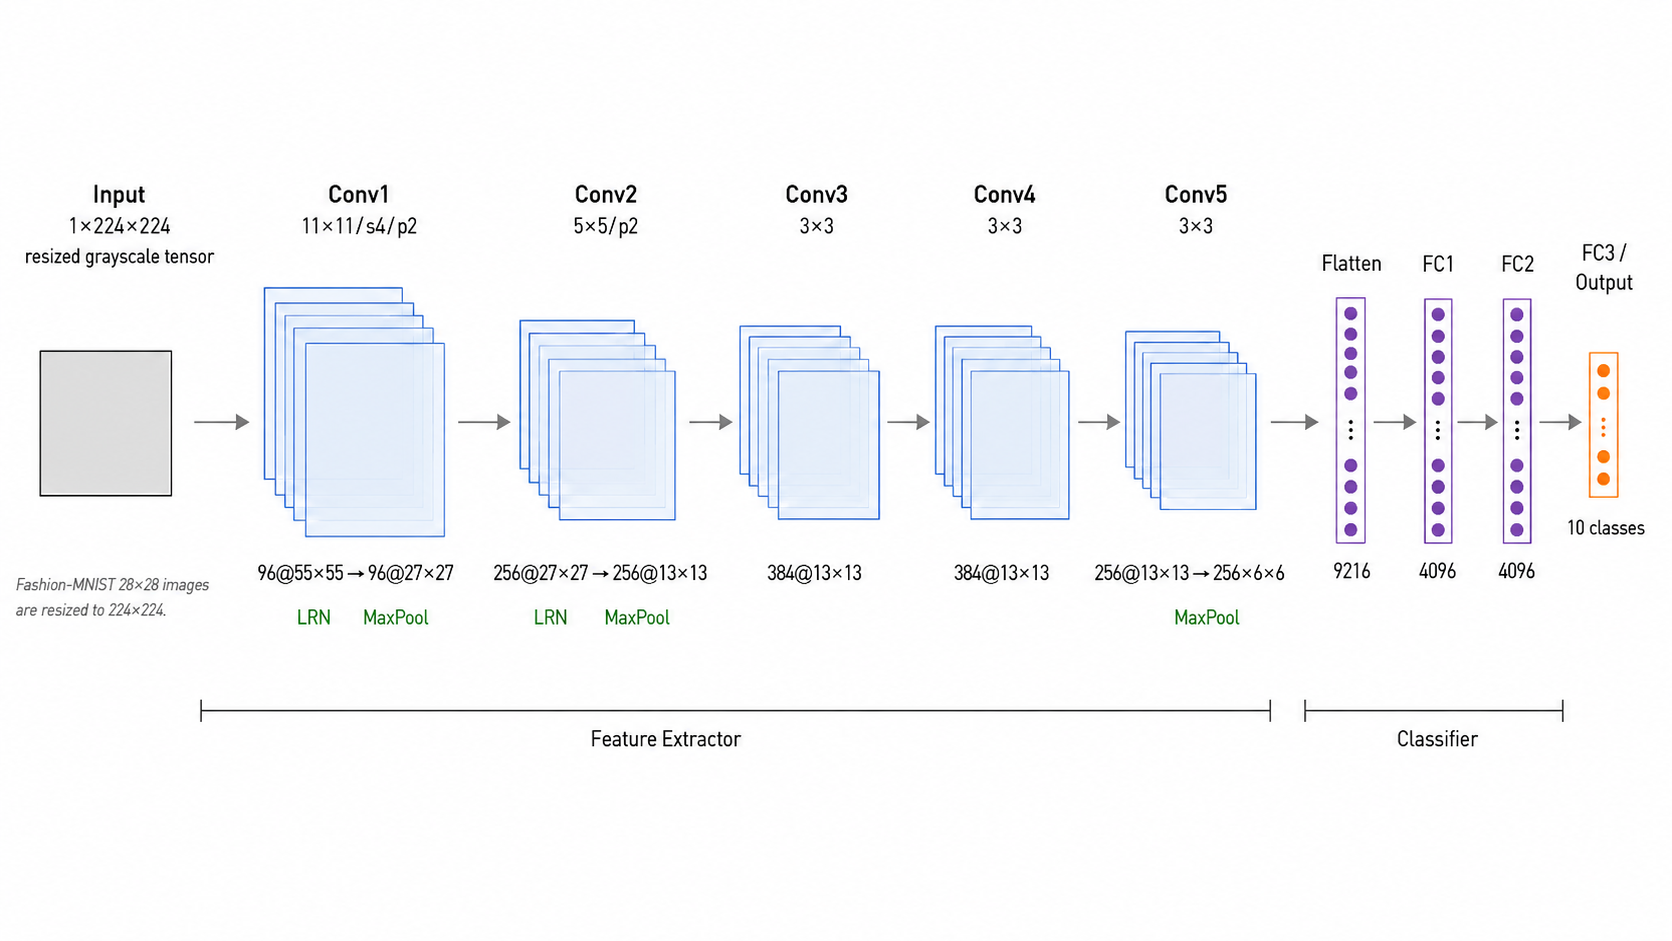
\includegraphics[width=0.95\textwidth]{fig_alexnet_arch.png}
  \caption{手写 AlexNet 网络结构示意}
  \label{fig:alexnet}
\end{figure}

\subsection{归一化、正则化与优化策略}
卷积网络训练不仅依赖结构本身，也依赖归一化、正则化和优化策略。原始 AlexNet 使用局部响应归一化（LRN）
增强相邻通道之间的竞争，但在后续深度学习实践中，Batch Normalization 更常用于稳定中间层输入分布。BatchNorm
通过 mini-batch 统计量对特征进行标准化，再引入可学习的缩放和平移参数：
\begin{equation}
\hat{x}=\frac{x-\mu_B}{\sqrt{\sigma_B^2+\epsilon}},\qquad y=\gamma\hat{x}+\beta.
\end{equation}
本文以 BatchNorm 作为主模型配置，并保留 LRN 基线作为对照，以分析归一化组件对训练稳定性和测试性能的影响。

Dropout 是 AlexNet 全连接分类器中的重要正则化手段。训练时随机置零一部分神经元输出，可以降低隐藏单元之间
的 co-adaptation，缓解大规模全连接层带来的过拟合风险。优化方面，本文采用带动量的 SGD。动量项能够累积历史
梯度方向，减少参数更新震荡；权重衰减通过惩罚过大的参数值控制模型复杂度；余弦退火学习率调度在训练后期逐步
降低学习率，有助于模型在较平滑的参数区域收敛。数据增强则通过随机水平翻转和小角度旋转构造输入扰动，提高
模型对轻微姿态变化的鲁棒性。

\subsection{评价指标}
本文采用准确率、宏平均精确率、宏平均召回率和宏平均 F1 评价多分类性能。宏平均指标对每个类别等权计算，
能够反映模型在不同类别上的平均表现。此外，本文还使用 ROC-AUC、Cohen's Kappa 和 MCC 等指标辅助评价，
并通过混淆矩阵分析具体错误类型。

准确率适合描述整体分类正确率，但当不同类别难度差异较大时，仅依赖准确率容易忽略局部错误。Fashion-MNIST
虽然类别数量均衡，但上装类别之间视觉相似，裤子、包、鞋类等类别则相对容易区分，因此宏平均 F1 更适合观察
每个类别的平均识别质量。Cohen's Kappa 扣除了随机一致性影响，MCC 综合考虑多分类混淆矩阵结构，二者可以从
一致性和相关性角度补充评价总体结果。ROC-AUC 则用于衡量模型概率输出对各类别的区分能力。除数值指标外，
本文将混淆矩阵、类别 F1 和 Grad-CAM 可视化结合起来分析错误来源，以避免只用单一分数评价模型。

\subsection{Grad-CAM 可解释性方法}
卷积网络的预测依据通常不如传统线性模型直观，因此需要借助可视化方法分析模型关注区域。Grad-CAM 利用目标类别
得分对最后一层卷积特征图的梯度，计算各通道对该类别的重要性权重：
\begin{equation}
\alpha_k^c=\frac{1}{Z}\sum_i\sum_j\frac{\partial y^c}{\partial A_{i,j}^k},
\end{equation}
其中 $A^k$ 表示第 $k$ 个特征图，$y^c$ 表示类别 $c$ 的得分，$Z$ 为空间位置数量。随后对加权特征图求和并经过
ReLU 得到类别激活图。该方法能够显示模型在作出某类预测时更关注图像中的哪些区域。本文使用 Grad-CAM 不是为了
替代定量指标，而是用于解释混淆矩阵中上装类别错误较多的可能原因。

% ===================== 第三章 数据集与模型实现 =====================
\section{数据集与模型实现}

\subsection{Fashion-MNIST 数据集}
Fashion-MNIST 数据集包含 70000 张 $28\times28$ 灰度服饰图像，其中训练集 60000 张、测试集 10000 张，覆盖
10 个类别：T 恤、裤子、套衫、连衣裙、外套、凉鞋、衬衫、运动鞋、包和短靴。本文从训练集中划分 10\% 作为
验证集，用于模型选择和训练过程监控。

该数据集的类别分布相对均衡，每类约 7000 张图像，能够减少类别数量不均衡对评价结果的干扰。但从视觉特征看，
不同类别的难度并不相同。裤子、包和鞋类在整体轮廓上具有明显差异，通常较容易识别；T 恤、套衫、外套和衬衫
均属于上装，低分辨率灰度图中缺少材质、颜色和细节纹理信息，类别边界更模糊。因此，本文后续重点分析上装类别
混淆，而不仅报告整体准确率。

\subsection{数据预处理}
由于 AlexNet 标准输入尺寸为 $224\times224$，本文通过 \texttt{Resize} 将 Fashion-MNIST 原图放大至
$224\times224$。随后使用 \texttt{ToTensor} 转换为张量，并根据 Fashion-MNIST 的单通道均值 0.2860 和标准差
0.3530 进行归一化。训练集可启用随机水平翻转和小角度旋转作为数据增强，验证集和测试集始终不使用随机增强。

将 $28\times28$ 图像放大至 $224\times224$ 并不会产生新的细节信息，但可以使输入尺寸与 AlexNet 经典结构保持
一致，避免重新设计卷积层和全连接层尺寸。该处理方式的代价是计算量显著增加，因此本文在第五章进行复杂度对比。
归一化操作能够稳定输入分布，使优化过程更平滑。数据增强只作用于训练集，验证集和测试集保持确定性变换，以保证
模型选择和最终评价不受随机增强影响。训练集划分验证集后，模型根据验证集表现保存最佳权重，再在测试集上进行
一次最终评估。

\begin{figure}[H]
  \centering
  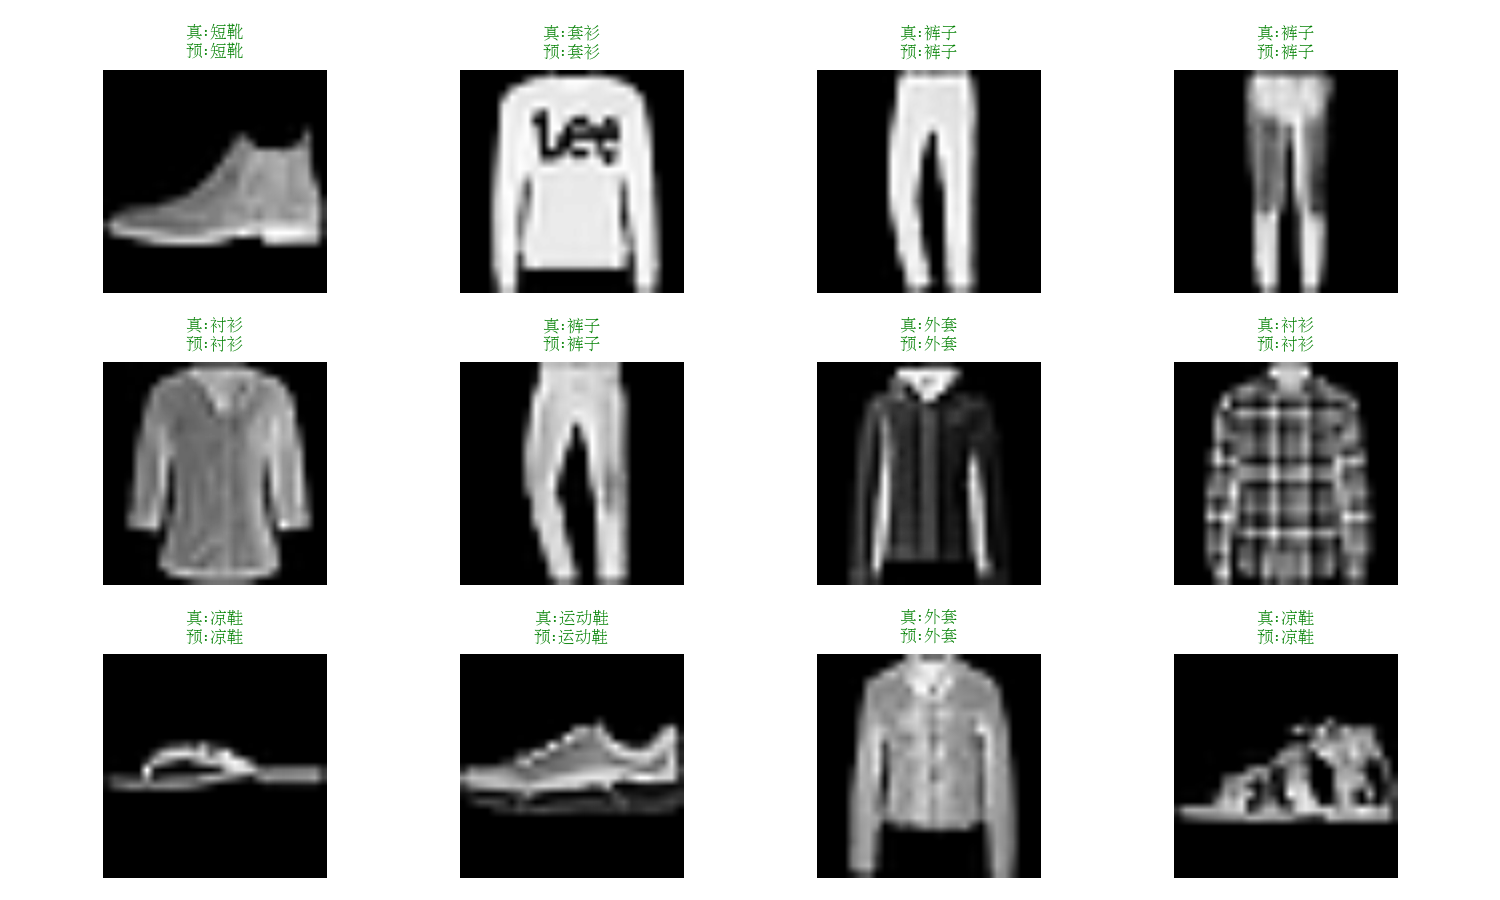
\includegraphics[width=0.88\textwidth]{samples.png}
  \caption{Fashion-MNIST 测试集预测样例}
  \label{fig:samples}
\end{figure}

\subsection{网络实现}
本文使用 PyTorch 基础模块逐层构建 AlexNet，核心模块包括卷积层、批归一化层、ReLU 激活、最大池化、
Dropout 和全连接层。实现过程中未调用预置 AlexNet 模型，而是通过基础算子手工搭建网络结构。主模型结构
如表~\ref{tab:structure} 所示。

网络前两层使用较大卷积核和最大池化快速扩大感受野并降低空间分辨率，后三个卷积层使用 $3\times3$ 卷积进一步
提取局部形状组合特征。最后一个池化层后，特征图尺寸降至 $256\times6\times6$，展平后输入三层全连接分类器。
全连接层前后加入 Dropout，以降低大容量分类器在训练集上过拟合的风险。本文在实现中显式记录每个模块输出尺寸，
用于检查网络结构是否与预期一致，也便于后续进行复杂度统计和实验复现。

\begin{table}[H]
  \centering
  \caption{主模型 AlexNet 结构}
  \label{tab:structure}
  \begin{tabular}{lll}
    \toprule
    模块 & 层结构 & 输出尺寸 \\
    \midrule
    Conv1 & $11\times11$ Conv, BN, ReLU, MaxPool & $96\times27\times27$ \\
    Conv2 & $5\times5$ Conv, BN, ReLU, MaxPool & $256\times13\times13$ \\
    Conv3 & $3\times3$ Conv, BN, ReLU & $384\times13\times13$ \\
    Conv4 & $3\times3$ Conv, BN, ReLU & $384\times13\times13$ \\
    Conv5 & $3\times3$ Conv, BN, ReLU, MaxPool & $256\times6\times6$ \\
    Classifier & Dropout, FC4096, FC4096, FC10 & 10 \\
    \bottomrule
  \end{tabular}
\end{table}

% ===================== 第四章 训练与评估 =====================
\section{训练与评估}

\subsection{训练设置}
主模型使用 SGD 优化器，动量为 0.9，权重衰减为 $5\times10^{-4}$，初始学习率为 0.01，批大小为 128，训练 40
轮，并采用余弦退火学习率调度。训练过程保存验证集准确率最高的模型权重，用于最终测试集评估。

训练流程包括前向传播、损失计算、反向传播、参数更新、验证集评估和最佳权重保存。损失函数采用多分类交叉熵，
其目标是提高真实类别的预测概率：
\begin{equation}
L=-\frac{1}{N}\sum_{i=1}^{N}\log p_{i,y_i}.
\end{equation}
训练过程中使用验证集准确率监控模型状态，而不是直接根据测试集调参。这样可以使测试集保持独立性，减少因反复
观察测试结果而造成的评价偏差。40 轮训练结合余弦退火调度，使模型在前期保持较大学习率进行充分搜索，后期逐渐
降低学习率以稳定收敛。

\begin{figure}[H]
  \centering
  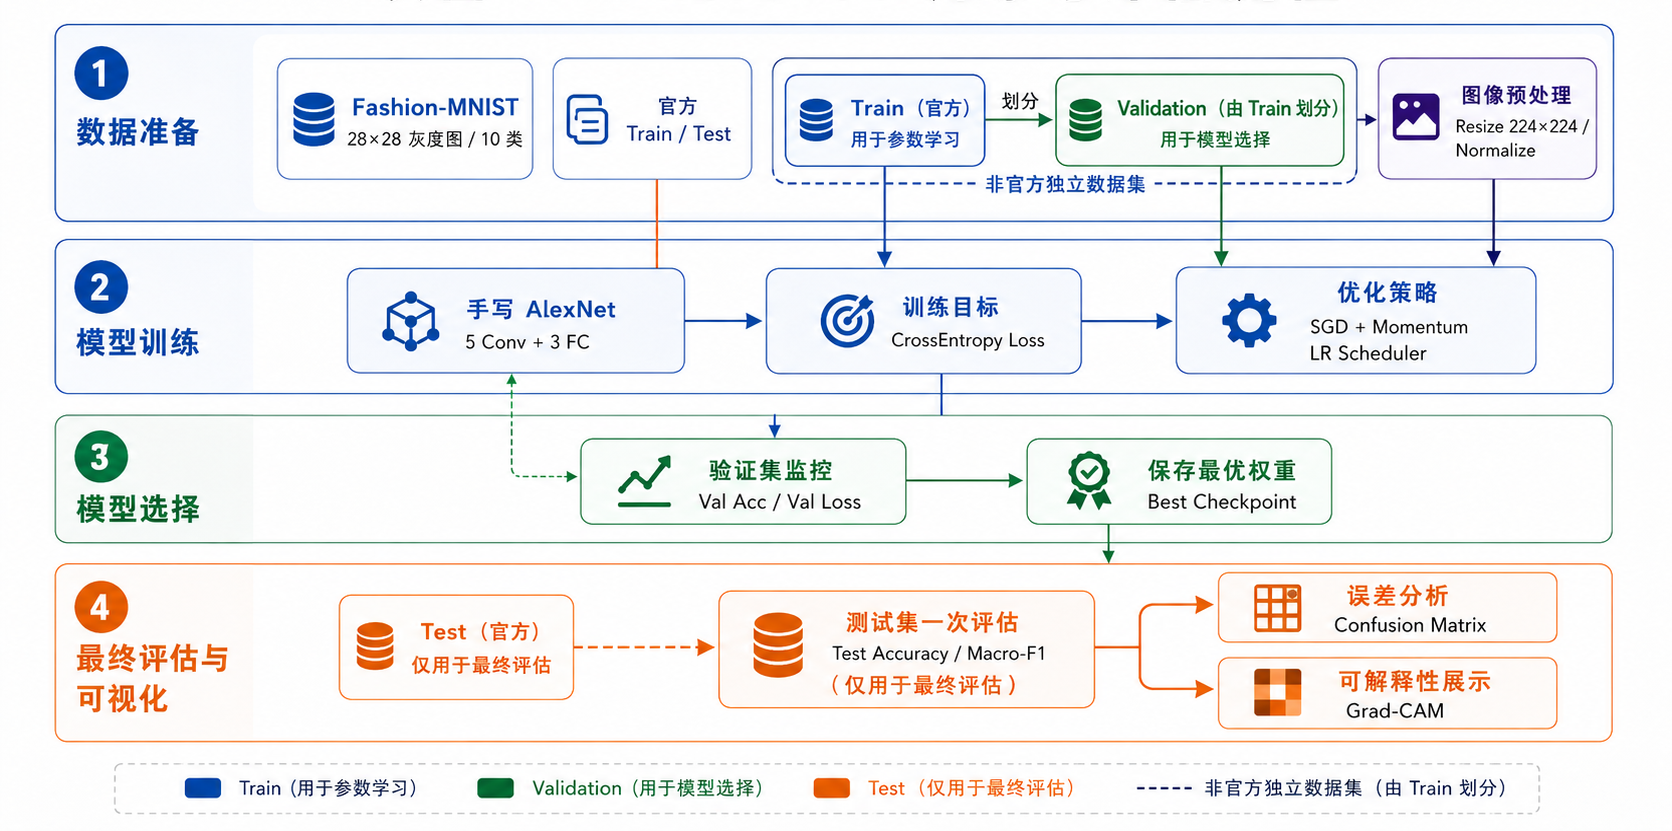
\includegraphics[width=0.95\textwidth]{fig_train_pipeline.png}
  \caption{任务二 AlexNet 训练与评估流程}
  \label{fig:train-pipeline}
\end{figure}

\begin{figure}[H]
  \centering
  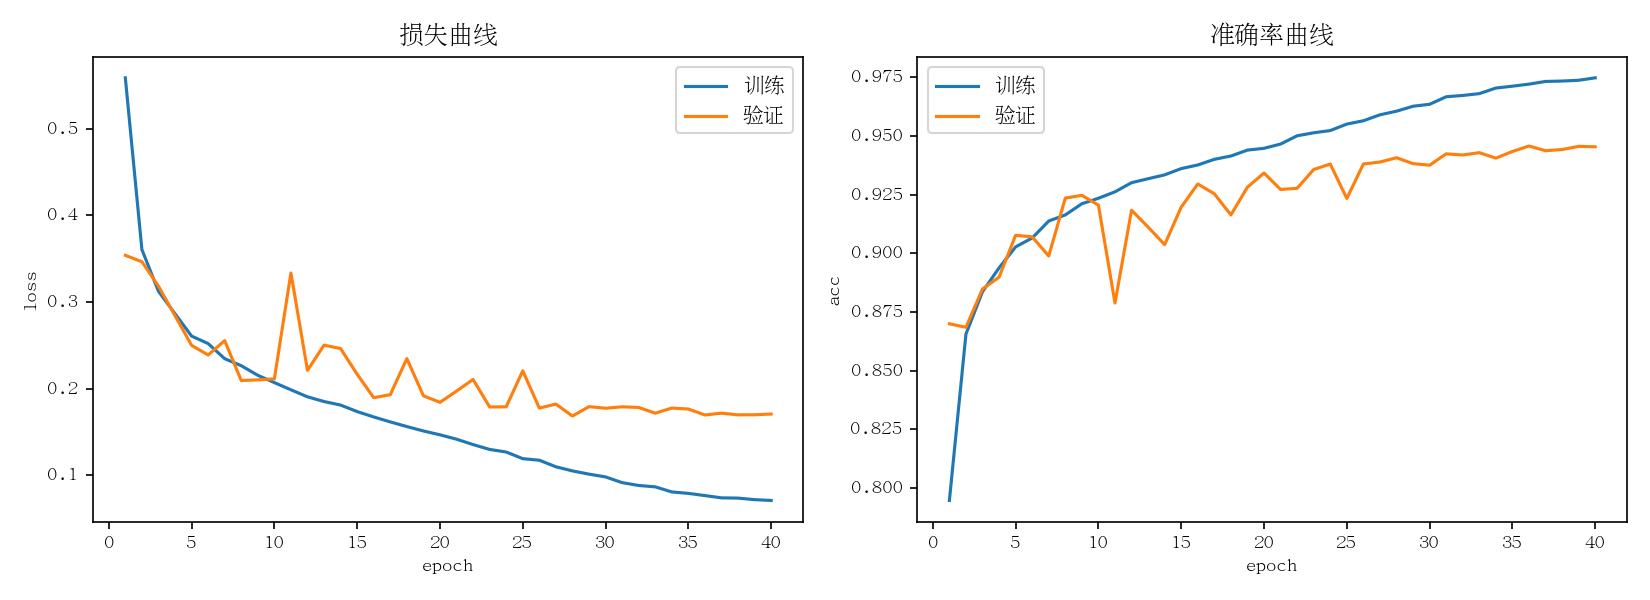
\includegraphics[width=0.86\textwidth]{curves.png}
  \caption{主模型训练与验证曲线}
  \label{fig:curves}
\end{figure}

从训练曲线看，主模型训练准确率和验证准确率整体随训练轮次上升，并在后期趋于稳定，说明模型已经完成较充分
训练。若训练轮次较少，AlexNet 的大容量分类器尚未充分收敛，容易出现测试性能偏低；而在 40 轮配置下，验证
曲线波动较小，说明 BatchNorm 和学习率调度对训练稳定性具有积极作用。由于训练集启用了数据增强，训练集指标
与验证集指标之间存在一定差异是正常现象，不能简单理解为模型退化。

\subsection{测试集结果}
主模型在 Fashion-MNIST 测试集上的整体结果如表~\ref{tab:test} 所示。模型最终准确率为 94.38\%，宏平均 F1
为 0.9437，说明手写 AlexNet 能够有效完成服饰图像十分类任务。

\begin{table}[H]
  \centering
  \caption{主模型测试集指标}
  \label{tab:test}
  \begin{tabular}{lccccc}
    \toprule
    准确率 & 宏精确率 & 宏召回率 & 宏 F1 & 宏 ROC-AUC & Cohen's Kappa \\
    \midrule
    0.9438 & 0.9437 & 0.9438 & 0.9437 & 0.9972 & 0.9376 \\
    \bottomrule
  \end{tabular}
\end{table}

\begin{figure}[H]
  \centering
  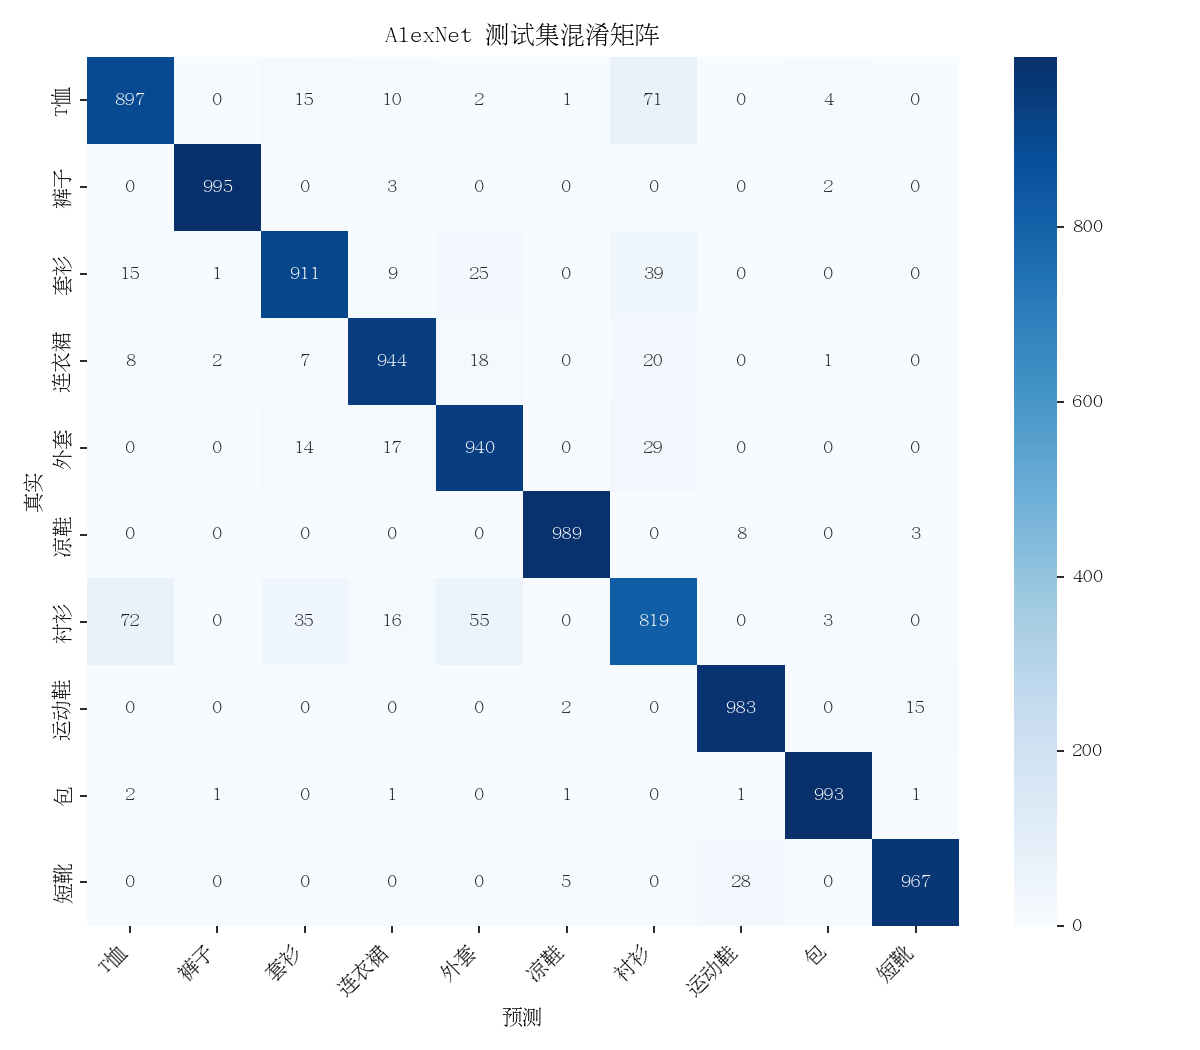
\includegraphics[width=0.72\textwidth]{confusion_matrix.png}
  \caption{主模型测试集混淆矩阵}
  \label{fig:cm}
\end{figure}

从混淆矩阵可以看出，裤子、鞋类和包等类别识别效果较好，而 T 恤、套衫、外套和衬衫之间仍存在较明显混淆。
这与 Fashion-MNIST 上装类别在低分辨率灰度图中视觉差异较小的特点相符。

宏平均精确率、宏平均召回率和宏平均 F1 均约为 0.944，说明模型在十个类别上的平均表现较均衡，并没有明显依赖
某个类别取得较高总体准确率。宏 ROC-AUC 达到 0.9972，表明模型概率输出在一对多意义下具有较强类别区分能力。
Cohen's Kappa 为 0.9376，说明预测结果与真实标签之间具有较高一致性。结合混淆矩阵可见，模型总体判别能力较强，
但其错误具有集中性：上装类别共享相似轮廓，且图像缺少颜色、材质和细节纹理，使得模型需要依赖袖口、衣摆、
领口等局部线索，而这些线索在 $28\times28$ 原图中并不总是清晰。

% ===================== 第五章 对照实验与误差分析 =====================
\section{对照实验与误差分析}

\subsection{组件消融实验}
为分析主模型性能来源，本文从 15 轮 LRN 基线出发，逐步加入充分训练、BatchNorm 和数据增强等设计。结果如
表~\ref{tab:improve} 和图~\ref{fig:improve} 所示。

\begin{table}[H]
  \centering
  \caption{AlexNet 组件消融实验结果}
  \label{tab:improve}
  \resizebox{\textwidth}{!}{%
  \begin{tabular}{lcccc}
    \toprule
    配置 & 测试准确率 & 宏平均 F1 & 衬衫类 F1 & 较上一行 \\
    \midrule
    最小配置（15 轮，LRN，无增强） & 0.9155 & 0.9153 & 0.77 & --- \\
    \quad + 充分训练（40 轮） & 0.9314 & 0.9312 & 0.79 & $+1.59$ \\
    \quad + BatchNorm 替代 LRN & 0.9432 & 0.9429 & 0.83 & $+1.18$ \\
    \quad\textbf{+ 数据增强（主模型）} & \textbf{0.9438} & \textbf{0.9437} & \textbf{0.83} & $\mathbf{+0.06}$ \\
    \bottomrule
  \end{tabular}}
\end{table}

\begin{figure}[H]
  \centering
  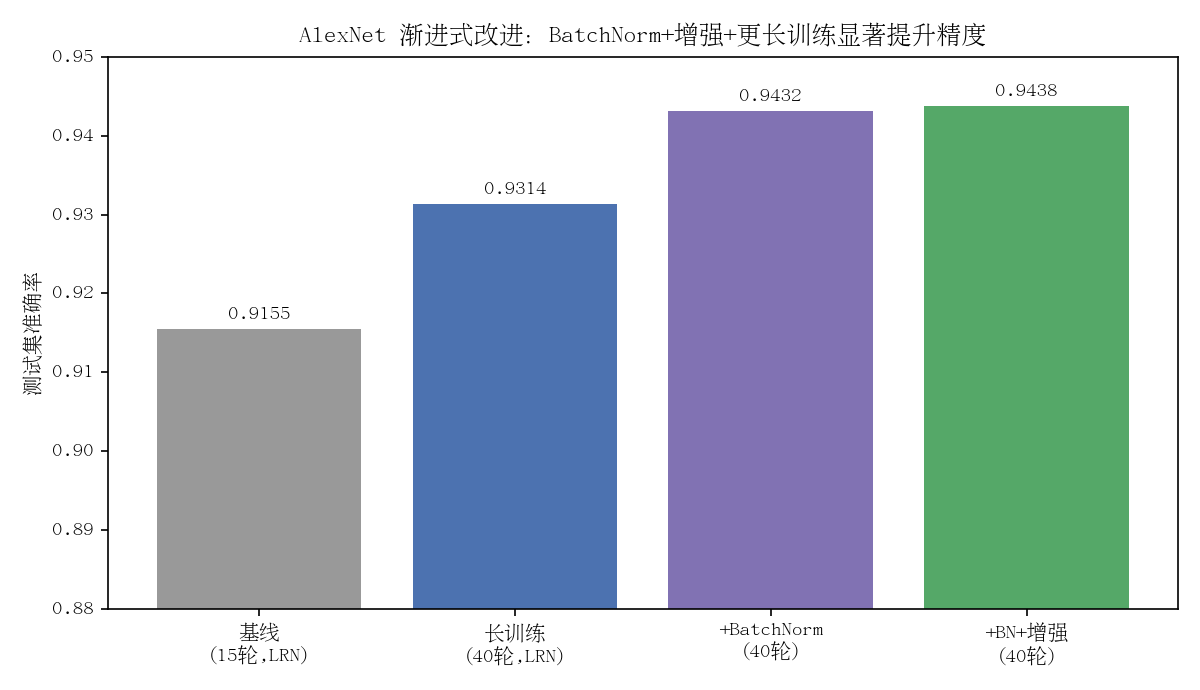
\includegraphics[width=0.72\textwidth]{improve_compare.png}
  \caption{组件消融实验结果对比}
  \label{fig:improve}
\end{figure}

消融实验表明，充分训练和 BatchNorm 对模型性能提升较明显；数据增强在 40 轮训练下带来小幅提升。该结果说明
训练预算、归一化组件和增强策略之间存在相互影响，不能脱离训练配置孤立评价某个组件。

具体来看，15 轮 LRN 基线测试准确率为 0.9155，延长至 40 轮并使用余弦退火后提升至 0.9314，说明原始训练预算
不足以充分发挥 AlexNet 的模型容量。进一步使用 BatchNorm 替代 LRN 后，准确率提升至 0.9432，衬衫类 F1 也由
0.79 左右提升到约 0.83，表明归一化组件对上装等较难类别具有明显帮助。加入数据增强后主模型准确率为 0.9438，
提升幅度较小，说明在当前增强强度和训练轮次下，增强主要起到轻微正则化作用，而不是性能提升的主要来源。
这一结果也提示，消融实验需要控制训练轮次、归一化方式和增强策略，否则容易把训练不充分误判为结构问题。

\subsection{模型复杂度对比}
AlexNet 参数量和计算量较大，而 Fashion-MNIST 图像分辨率较低。本文进一步比较 AlexNet 与轻量 SimpleCNN 的
复杂度，结果如表~\ref{tab:complexity} 所示。

\begin{table}[H]
  \centering
  \caption{AlexNet 与 SimpleCNN 复杂度对比}
  \label{tab:complexity}
  \resizebox{\textwidth}{!}{%
  \begin{tabular}{lcccc}
    \toprule
    模型 & 参数量 & 单图 FLOPs & GPU 单图延迟 & CPU 单图延迟 \\
    \midrule
    AlexNet@224 & 58.302M & 1063.5M & 0.765 ms & 15.437 ms \\
    SimpleCNN@28 & 0.391M & 7.9M & 0.452 ms & 1.496 ms \\
    倍数 & 149.1$\times$ & 134.6$\times$ & 1.7$\times$ & 10.3$\times$ \\
    \bottomrule
  \end{tabular}}
\end{table}

复杂度结果表明，AlexNet 在该任务上存在一定参数和计算冗余。为进一步验证架构选择的影响，本文还对比了手写
小型 ResNet。结果显示，小型 ResNet 在测试准确率上达到 94.92\%，略高于 AlexNet，同时参数量明显更小。

AlexNet@224 的参数量约为 58.302M，是 SimpleCNN@28 的 149.1 倍；单图 FLOPs 约为 1063.5M，是 SimpleCNN 的
134.6 倍。GPU 单图延迟差距相对较小，说明并行计算可以部分抵消大模型计算开销；但 CPU 单图延迟达到
SimpleCNN 的 10.3 倍，更能体现模型部署成本。考虑到 Fashion-MNIST 原图只有 $28\times28$，将图像放大并使用
大规模全连接分类器并不一定是效率最优选择。小型 ResNet 的对照结果进一步说明，现代结构可以在更少参数下取得
接近或略高性能。不过，本文保留 AlexNet 作为主模型，是为了围绕经典卷积网络完成逐层实现、训练和分析，而复杂度
结果则用于客观说明其在该任务上的效率局限。

\begin{figure}[H]
  \centering
  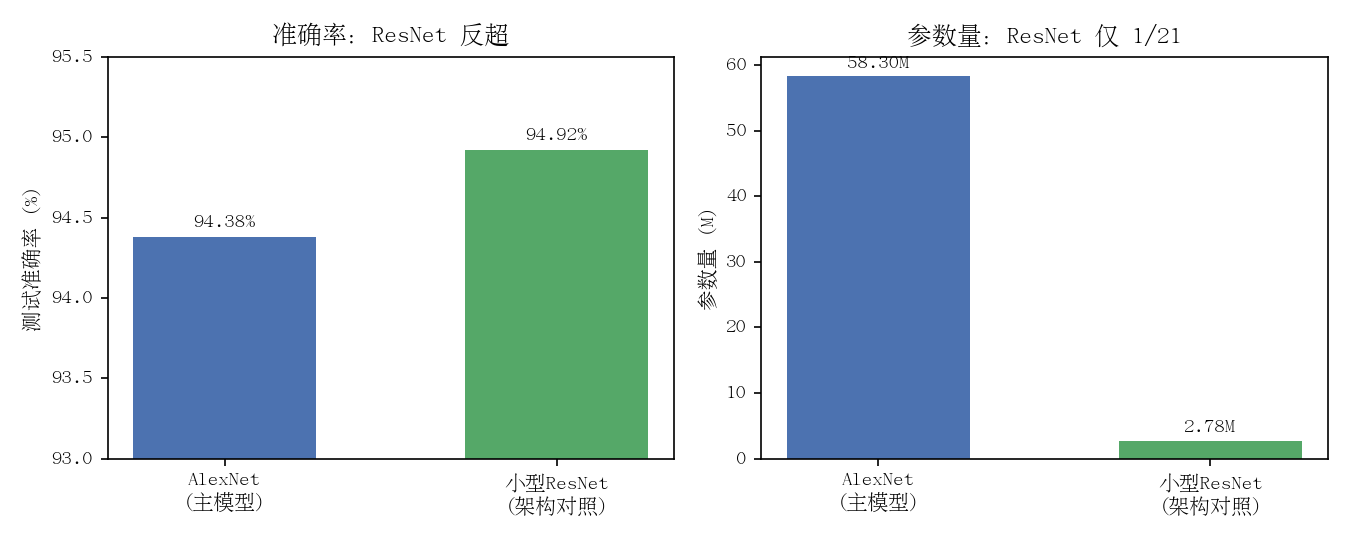
\includegraphics[width=0.72\textwidth]{arch_compare.png}
  \caption{AlexNet 与小型 ResNet 架构对照}
  \label{fig:arch}
\end{figure}

\subsection{Focal Loss 与 Grad-CAM 分析}
为分析上装类别混淆是否来自难分样本加权不足，本文比较了交叉熵损失与 Focal Loss。结果如表~\ref{tab:focal}
所示，在该实验配置下 Focal Loss 未优于交叉熵损失，说明主要困难更可能来自类间视觉特征相似，而不是样本
数量不均衡。

\begin{table}[H]
  \centering
  \caption{Focal Loss 与交叉熵对照实验}
  \label{tab:focal}
  \begin{tabular}{lcccc}
    \toprule
    损失函数 & 测试准确率 & 宏平均 F1 & 衬衫类 F1 & 裤子类 F1 \\
    \midrule
    交叉熵 & 0.9247 & 0.9245 & 0.78 & 0.97 \\
    Focal Loss & 0.9167 & 0.9163 & 0.75 & 0.86 \\
    \bottomrule
  \end{tabular}
\end{table}

\begin{figure}[H]
  \centering
  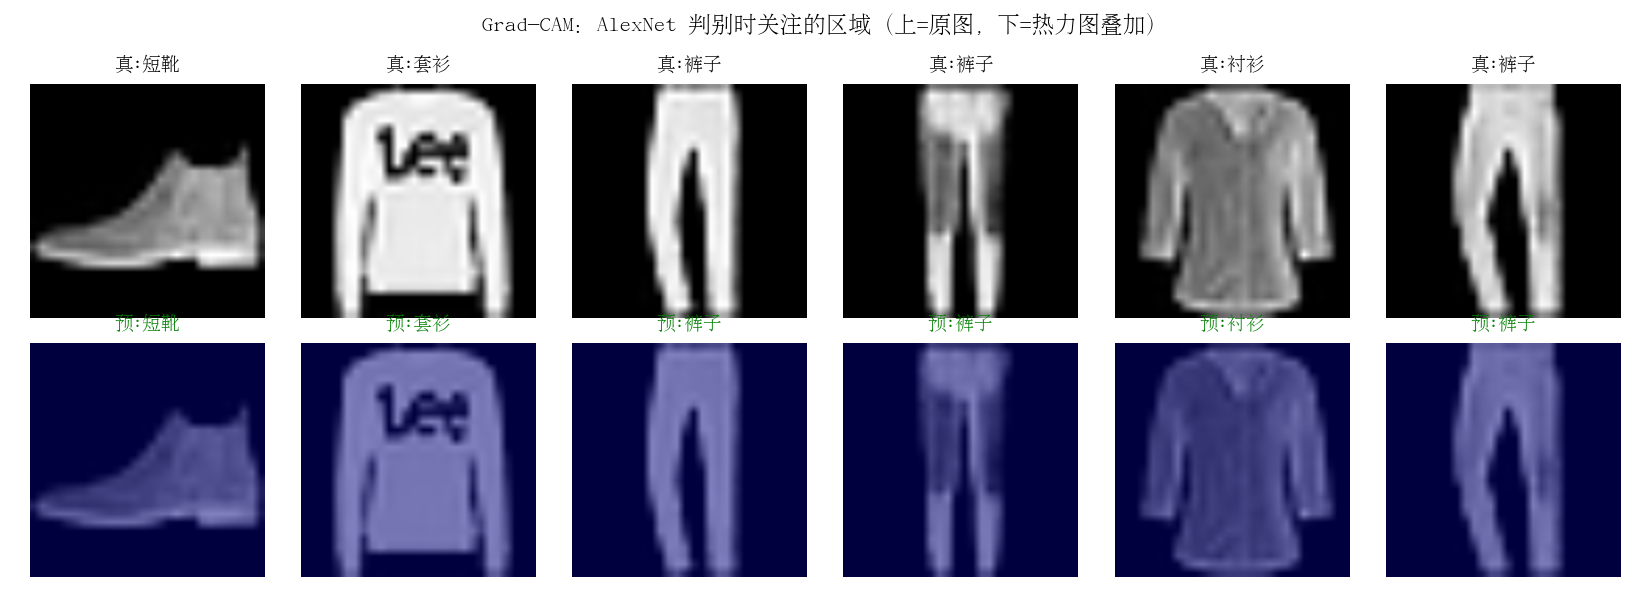
\includegraphics[width=0.82\textwidth]{gradcam.png}
  \caption{Grad-CAM 可解释性可视化}
  \label{fig:gradcam}
\end{figure}

Grad-CAM 结果显示，模型注意力主要落在服饰主体轮廓，对区分上装所需的细粒度局部区域关注不足。这一结果与
混淆矩阵和 Focal Loss 对照相互印证，支持“上装类别错误主要来自细粒度特征表达不足”的分析。

Focal Loss 通常用于类别极不均衡或易分样本占比过高的场景，其核心思想是降低易分样本的损失权重，使模型更关注
难分样本。但 Fashion-MNIST 类别数量相对均衡，本实验中上装错误更多来自视觉差异不足和局部细节缺失，而不是
少数类别样本数量不足。因此，Focal Loss 在当前配置下准确率和宏平均 F1 均低于交叉熵，并不意外。该结果说明，
面对错误类别时，应先判断错误来源是样本不均衡、训练不足、结构容量不足，还是输入信息本身有限，再选择相应改进
方法。

Grad-CAM 可视化进一步补充了这一判断。若模型主要关注服饰整体轮廓，它能够较好区分裤子、包和鞋类等轮廓差异
明显的类别；但对于 T 恤、套衫、外套和衬衫，决定类别的线索往往位于领口、袖长、开襟、衣摆等局部区域。低分辨率
灰度图中这些细节较弱，模型即使关注主体区域，也可能缺少足够信息完成稳定区分。因此，后续改进可以考虑更适合
小图像的网络结构、局部注意力机制或更强的数据增强策略，而不是单纯增加损失函数复杂度。

% ===================== 第六章 实验复现说明 =====================
\section{实验复现说明}

\subsection{代码结构}
任务二源代码和主要输出文件如表~\ref{tab:code} 所示。
\begin{table}[H]
  \centering
  \caption{任务二源代码与输出文件说明}
  \label{tab:code}
  \begin{tabular}{ll}
    \toprule
    文件 & 功能 \\
    \midrule
    alexnet.py & 逐层手写 AlexNet 网络定义 \\
    data.py & Fashion-MNIST 数据加载、预处理与划分 \\
    experiments.py & 主模型与对照实验统一运行器 \\
    evaluate.py & 测试集评估、曲线、混淆矩阵与样例图生成 \\
    aggregate\_experiments.py & 对照实验结果聚合与绘图 \\
    gradcam.py & Grad-CAM 可解释性可视化 \\
    complexity.py & 参数量、FLOPs 和推理延迟统计 \\
    \bottomrule
  \end{tabular}
\end{table}

\subsection{运行步骤}
在项目根目录下执行以下命令训练主模型：
\begin{quote}
{\small\ttfamily
python task2\_alexnet\_fmnist/experiments.py --model alexnet \textbackslash\newline
\hspace*{2em}--bn --augment --cosine --epochs 40 --seed 0 --tag main \textbackslash\newline
\hspace*{2em}--save-ckpt task2\_alexnet\_fmnist/outputs/alexnet\_best.pt \textbackslash\newline
\hspace*{2em}--save-history task2\_alexnet\_fmnist/outputs/history.json}
\end{quote}
随后执行以下命令完成测试集评估：
\begin{quote}
{\small\ttfamily python task2\_alexnet\_fmnist/evaluate.py}
\end{quote}
对照实验可通过不同的 \texttt{--model}、\texttt{--bn}、\texttt{--augment}、\texttt{--loss} 和
\texttt{--epochs} 参数组合运行，并使用 \texttt{aggregate\_experiments.py} 汇总。

% ===================== 第七章 结论与展望 =====================
\section{结论与展望}

\subsection{结论}
本文基于 PyTorch 基础模块逐层实现 AlexNet，并在 Fashion-MNIST 十分类任务上完成训练和评估。主模型在测试集
上取得 94.38\% 的准确率和 0.9437 的宏平均 F1，说明 AlexNet 能够有效完成服饰图像分类任务。误差分析显示，
模型主要混淆集中在视觉相似的上装类别之间。消融实验表明，充分训练和 BatchNorm 对性能提升具有较大作用；
复杂度分析则说明 AlexNet 在低分辨率灰度图像任务上存在一定冗余。Grad-CAM 可视化进一步揭示模型主要关注
服饰整体轮廓，对细粒度局部差异的利用仍有限。

从实验完整性看，本文不仅完成了主模型训练，还围绕训练策略、归一化组件、数据增强、损失函数、模型复杂度和
可解释性进行了多角度分析。结果表明，AlexNet 的经典卷积结构仍然能够在 Fashion-MNIST 上取得较高识别性能；
但在低分辨率灰度服饰图像上，性能瓶颈主要集中在上装细粒度区分和模型效率两个方面。这样的结果有助于理解
经典 CNN 结构的优势与局限，也为后续选择更轻量或更适合小图像的网络提供了依据。

\subsection{不足与展望}
本文仍存在一些不足。首先，AlexNet 参数量较大，与 Fashion-MNIST 任务规模并不完全匹配；其次，部分对照实验
只采用单随机种子，后续可进行更多重复实验以评估稳定性；最后，可进一步引入 VGG、ResNet、轻量 CNN 等架构，
系统比较不同网络在低分辨率服饰图像分类任务上的性能、计算开销和可解释性。

后续工作可以从三个方向展开。第一，在实验设计上增加多随机种子重复训练，报告均值和标准差，以降低单次训练
波动对结论的影响。第二，在模型结构上比较适配 $28\times28$ 小图像的轻量 CNN、ResNet 变体或注意力模块，避免
因强行放大输入造成不必要计算。第三，在误差分析上进一步收集错误样本，结合类别原型、局部遮挡和更系统的
可解释性方法，分析上装类别混淆是否可以通过局部特征增强得到改善。这样可以使后续研究从“模型能否分类”进一步
推进到“模型为什么会错、怎样更有效地改进”。

% ===================== 参考文献 =====================
\section*{参考文献}
\addcontentsline{toc}{section}{参考文献}
{\setlength{\parindent}{0pt}
\newcommand{\refentry}[1]{\par\hangindent=2em\hangafter=1 #1\vspace{3pt}}
\refentry{He K, Zhang X, Ren S, et al. Deep residual learning for image recognition[C]//IEEE Conference on Computer Vision and Pattern Recognition. 2016: 770-778.}
\refentry{Ioffe S, Szegedy C. Batch normalization: accelerating deep network training by reducing internal covariate shift[C]//International Conference on Machine Learning. 2015: 448-456.}
\refentry{Krizhevsky A, Sutskever I, Hinton G E. ImageNet classification with deep convolutional neural networks[C]//Advances in Neural Information Processing Systems. 2012: 1097-1105.}
\refentry{LeCun Y, Bottou L, Bengio Y, et al. Gradient-based learning applied to document recognition[J]. Proceedings of the IEEE, 1998, 86(11): 2278-2324.}
\refentry{Lin T Y, Goyal P, Girshick R, et al. Focal loss for dense object detection[C]//IEEE International Conference on Computer Vision. 2017: 2980-2988.}
\refentry{Paszke A, Gross S, Massa F, et al. PyTorch: an imperative style, high-performance deep learning library[C]//Advances in Neural Information Processing Systems. 2019: 8024-8035.}
\refentry{Selvaraju R R, Cogswell M, Das A, et al. Grad-CAM: visual explanations from deep networks via gradient-based localization[C]//IEEE International Conference on Computer Vision. 2017: 618-626.}
\refentry{Simonyan K, Zisserman A. Very deep convolutional networks for large-scale image recognition[C]//International Conference on Learning Representations. 2015.}
\refentry{Srivastava N, Hinton G, Krizhevsky A, et al. Dropout: a simple way to prevent neural networks from overfitting[J]. Journal of Machine Learning Research, 2014, 15(1): 1929-1958.}
\refentry{Xiao H, Rasul K, Vollgraf R. Fashion-MNIST: a novel image dataset for benchmarking machine learning algorithms[J]. arXiv preprint arXiv:1708.07747, 2017.}
}

\end{document}
